%\RequirePackage{lineno}
\documentclass[aps,prc,preprint,superscriptaddress,showpacs,showkeys]{revtex4-1}
\usepackage{graphicx}
\begin{document}
\newcommand{\Jpsi}{J/\psi}
\newcommand{\pT}{p_{T}}

%\linenumbers
\title{{\Large Quarkonia suppression in PbPb collisions at $\sqrt s_{NN}$ =  2.76 TeV }}
\author{\large Vineet Kumar}
\author{\large Prashant Shukla}
\email{pshukla@barc.gov.in}
\affiliation{Nuclear Physics Division, Bhabha Atomic Research Center, Mumbai, India}
\affiliation{Homi Bhabha National Institute, Anushakti Nagar, Mumbai, India}
\date{\today}

\begin{abstract}
  We calculate the quarkonia yield modification in the medium produced in PbPb
collisions at LHC energy. We use a kinetic model which incorporates quarkonia yield 
modifications due to suppression inside QGP, suppression due to hadronic comovers and 
regeneration of quarkonia from charm pairs. 
 Quarkonia dissociation cross section due to gluon collisions has been considered and
the regeneration rate has been obtained using the principle of detailed balance.
 Modification in yield due to comovers has been estimated assuming it to be caused by
pion collisions.  
  The nuclear modification factors in PbPb collisions at $\sqrt s_{NN}$ =  2.76 TeV for 
both $\Jpsi$ and $\Upsilon$ have been measured at different centralities and transverese 
momenta by different experiments. The calculations are carried in same measured kinematic 
regions to study the menifestation of medium effects in comparison with the measured data.
 Both the suppression and regeneration strongly affect $\Jpsi$ yields in low $\pT$ range 
and the large high $\pT$ suppression of $\Jpsi$ is much more than what is expected by 
gluon dissociation.
\end{abstract}

\pacs{12.38.Mh, 24.85.+p, 25.75.-q}
\keywords{quark-gluon plasma, quarkonia, suppression, regeneration}
\maketitle
%%%%%%%%%%%%%%%%%%%%%%%%%%%%%%%%%%%%%%%%%%%%%%%%%%%%%%%%%%%%%%%%%%%%%%%%%%%%%%%%%%%%%%%%%%%%%%%%%%%%%%%%%%%%%%%%%
\section{Introduction}
  Heavy ion collisions at relativistic energies are performed to create and characterize 
Quark Gluon plasma (QGP), a phase of strongly interacting matter at an energy density 
where quarks and gluons are no longer bound within hadrons. 
  Quarkonia state ($\Jpsi$ and $\Upsilon$) have been one of the most popular tools 
since their suppression was proposed as a signal of QGP \cite{SATZ}.
  The understanding of these probes has evolved substantially via measurements 
through three generations of experiments: SPS (at CERN), RHIC (at BNL) and the LHC (at CERN) 
and by voluminous theoretical activities [For a recent reviews see 
Refs.~\cite{Schukraft,Kluberg:2009wc,Brambilla:2010cs,Rapp:2008tf}].

 The quarkonia are produced early in the heavy ion collisions and if they evolve
through deconfined medium their yields should be suppressed in comparison with $pp$. 
 The first such measurement was 'anomalous' $\Jpsi$ suppression discovered at the SPS 
which was considered as a hint of QGP formation. The RHIC results showed almost the same suppression at 
a much higher energy contrary to the expectation \cite{Brambilla:2010cs}. The suggestion then followed was 
the anomalous suppression could well be due to dissociation of excited charmonia states by 
hadronic interactions at both energies not requiring QGP.   
  It was also suggested that at higher collision energy the expected more suppression is 
compensated by regeneration of $\Jpsi$ by the recombination of two 
independently produced charm quarks~\cite{Andronic_SH1}.

  After the LHC started PbPb collisions at $\sqrt s_{NN} = 2.76$ TeV, wealth of
results have become available on quarkonia production \cite{QGP_Tc}. 
  The CMS experiment carries out $\Jpsi$ measurement at high transverse momentum 
($p_T>6.5$ GeV/$c$). The high $p_T$ prompt $\Jpsi$ is found to be suppressed substantially
even in peripheral collisions with nuclear modification factor $R_{AA}$ decreasing as a function 
of increasing centrality \cite{JCMS,CMSJPsi}. 
  Moreover the $R_{AA}$ is found to be nearly independent of $p_T$ (above 6 GeV$/c$) showing 
that $\Jpsi$ remain suppressed even at very high $p_T$ upto 15 GeV/$c$.
 On comparing with STAR results \cite{STARjpsi} at RHIC it follows that the suppression of
 $\Jpsi$ has increased with collision energy.
  The ALICE results \cite{ALICEJPsi} of $\Jpsi$ covers low $p_T$ and are complementary 
to CMS measurements.
  The suppression of low $p_T$  $\Jpsi$ is found to have little or no centrality 
dependence.  When compared with PHENIX forward rapidity measurement at 
RHIC \cite{PHENIXJPsi}, it suggests that low p$_T$ $\Jpsi$ are less suppressed at LHC.
 The ALICE results also showed that $\Jpsi$ suppression decrease substantially with 
decreasing $p_T$ and at very low $p_T$ the suppression is small.
 It is consistent with the picture of regeneration of $\Jpsi$ at low $p_T$
compensating the suppression due to deconfinement ~\cite{ALICEJPsi}. 
The bottomomia states are also measured by CMS \cite{CMSUpsilon1,CMSUpsilon2} and
ALICE \cite{ALICEUpsilon} experiments at LHC. CMS measurement is in mid rapidity region
($|y^{\Upsilon}|\,\leq 2.4$) while ALICE measured in forward rapidity ($2.5 \leq y^{\Upsilon} \leq 4.0$).  
Both measurements matches within uncertanity and CMS experiment that the excited $\Upsilon$ 
are more suppressed relative to the ground state.
  The quarkonium states with more binding energy should show less suppresion, 
a phenomenon referred as sequential suppression first time observed at LHC.  
  Many theoertical framework have been developed in pre-LHC years for the modification of 
quarkonia due to different processes. 
 The suppression of quarkonia in QGP are understood in terms of colour screening models  
e.g. Ref. \cite{SATZ,YSuppAbdShuk} and the dissociation of quarkonia by gluon
collision process \cite{BhanotPeskin,Xu}. The statistical models \cite{Andronic_SH1,Andronic_SH2}
offer estimates of the regeneration of quarkonia from a charm quark pairs.
Inverse of gluon dissociation process is also used to estimate regeneration \cite{Grandchamp,Thews}.  
  The quarkonia yields in heavy ion collisions are also modified due to non-QGP effects such as
shadowing, an effect due to change of the parton distribution functions inside the nucleus,
and dissociation due to hadronic or comover interaction \cite{Vogt}.
 There have been many recent calculations to explain the LHC results on quarkonia using a 
combination of above theoretical frameworks and models \cite{Rapp1,Rapp2}. 

 In this paper, we calculate the quarkonia (both $\Jpsi$ and $\Upsilon$) suppression 
due to thermal gluon dissociation in an expanding Quark Gluon Plasma. 
Other sources which can suppress the yield are considered e.g. nuclear shadowing and 
comover interaction. We also include the effect of $\Jpsi$ regeneration estimated from 
inverse of gluon dissociation process using the principle of detailed balance. 
The nuclear modification factor of $\Jpsi$ is obtained as a function of transverse momentum 
and centrality of collision. Calculations are compared with experimental data from CMS 
and ALICE.

 


\section{Heavy quark production rates}
The production cross sections for heavy quark pairs are calculated to NLO in pQCD  
using the CTEQ6M parton densities \cite{CTEQ6}.  The central EPS09 parameter set 
\cite{EPS09} is used to calculate the modifications of the parton densities in 
Pb+Pb collisions.  We use the same set of parameters
as that of Ref.~\cite{CNV} with the NLO calculation of Ref.~\cite{MNR}
to obtain the exclusive $Q \overline Q$ pair rates as well as their decays
to dileptons.  
 The production cross sections for heavy flavor and quarkonia at $\sqrt{s_{_{NN}}}= 2.76$ 
TeV \cite{ContinuumVKShuk} are given in Table~\ref{NLOcros}.  The number of $Q \overline Q$ pairs
in a minimum bias Pb+Pb event is obtained from the per nucleon cross
section, $\sigma_{\rm PbPb}$, by
\begin{eqnarray}
N_{Q \overline Q} = {A^2 \sigma_{\rm PbPb}^{Q \overline Q}  \over  
\sigma_{\rm PbPb}^{\rm tot}} \, \, .
\end{eqnarray}
 At 2.76 TeV, the total Pb+Pb cross section, $\sigma_{\rm PbPb}^{\rm tot}$, 
is 7.65 b \cite{PbPbTotal}.

\begin{table}
\caption[]{Heavy quark and quarkonia cross sections at
$\sqrt{s_{_{NN}}}= 2.76$ TeV. The cross sections are given per nucleon pair while
$N$ gives number of heavy quark pair/quarkonia per Pb+Pb event.}
\label{NLOcros}
\begin{tabular}{l|l|l|l|l} 
\hline 
\hline
                     & $ c \overline c$           &$\Jpsi$      & $ b \overline b$           & $\Upsilon$   \\              
\hline
$\sigma_{\rm PbPb}$  & $1.76^{+2.32}_{-1.29}$ mb  & $31.4 \mu$b  & $89.3^{+42.7}_{-27.2} \mu$b  & $0.38 \mu$b  \\
$N$                  &$9.95^{+13.10}_{-7.30}$     & $0.177$      & $0.50^{+0.25}_{-0.15}$     & $0.01$       \\
\hline
\hline
\end{tabular}
\end{table}





%%%%%%%%%%%%%%%%%%%%%%%%%%%%%%%%%%%%%%%%%%%%%%%%%%%%%%%%%%%%%%%%%%%%%%%%%%%%%%%%%%%%%%%%%%
\section{Modification of quarkonia in the presence of QGP}
 In Kinetic approach \cite{Thews} the proper time ($\tau$) evolution of the $\Jpsi$ population is given 
by the rate equation 

\begin{equation}\label{eqkin}
{dN_{\Jpsi} \over d\tau}  =  - \lambda_D  \rho_g N_{\Jpsi} + \lambda_F {N_{c \bar{c}}^{2} \over V(\tau)},
\end{equation}
where $V(\tau)$ is the volume of the deconfined spatial region and $N_{c \bar{c}}$ is the number of initial 
charm quark pairs produced per event.
 The $\lambda_{D}$ is the dissociation rate obtained by the cross-section averaged over the momentum 
distribution of gluons and $\lambda_{F}$ is the regeneration rate obtained by the cross-section 
averaged over the momentum distribution of $c$ and $\bar c$. $\rho_g$ is the density of thermal gluons.
 The number of $\Jpsi$ at freeze-out time $\tau_f$ is given by solution of Eq.~(\ref{eqkin}) 
\begin{equation}
N(p_T) = S(p_T) \,N_{\Jpsi}^{0}(p_T)+N_{\Jpsi}^{\rm regen}(p_T).
\label{eqbeta}
\end{equation}
Here $N_{\Jpsi}^{0}(p_T)$ is the number of initially produced $\Jpsi$ as a function of $p_T$ and 
$S(p_T)$ is their survival probability from gluon collisions at freeze-out time $\tau_f$ and 
is written as
\begin{equation}
S(\tau_f,p_T) = \exp \left( {-\int_{\tau_0}^{\tau_f}f(\tau) \lambda_{\rm D}(T,p_T)\,\rho_g(T)\,d\tau} \right).
\end{equation}
The temperature $T(\tau)$ and the QGP fraction $f(\tau)$ evolve from initial time $\tau_0$ to freeze-out time
$\tau_f$ due to expansion of QGP.
$N_{\Jpsi}^{\rm regen}(p_T)$ is the number of regenerated $\Jpsi$ per event and is given by
\begin{equation}
N_{\Jpsi}^{\rm regen}(p_T)=S(\tau_f,p_T)N_{c \bar{c}}^{2} \int_{\tau_0}^{\tau_f}{{\lambda_{\mathrm{F}} \over V(\tau)\,S(\tau,p_T)} d\tau}
\end{equation}

   The nuclear modification factor ($R_{AA}$) can be written as 
\begin{equation}
R_{AA}(p_T)=S(p_T) + \frac{N_{\Jpsi}^{\rm regen}(p_T)}{N_{\Jpsi}^{0}(p_T)}
\label{raa}
\end{equation}
$R_{AA}$ as a function of collision centrality, including the regeneration will be  
\begin{equation}
R_{AA}(N_{\rm part}) = \frac{\int_{p_{T\,\rm Cut}} N_{\Jpsi}^{0}(p_T)S(p_T)dp_T}{\int_{p_{T\,\rm Cut}} N_{\Jpsi}^{0}(p_T) dp_T} + 
\frac{\int_{p_{T\, \rm Cut}} N_{\Jpsi}^{\rm regen}(p_T) dp_T}{\int_{p_{T\, \rm Cut}} N_{\Jpsi}^{0}(p_T) dp_T}
\label{raa2}
\end{equation}
Here $p_{\rm Cut}$ defines the $p_T$ range as per the experimental measurements.
 $N_{\Jpsi}^{0}(p_T)$ is the unmodified $p_T$ distribution of $\Jpsi$ calculated by Pythia \cite{Pythia1,Pythia2}. 

 The temperature evolution for different centralities of collision is obtained by 
assuming an isentropical cylindrical expansion with volume element
\begin{equation}
V(\tau) = \tau\,\pi\,(R_0 + {1\over 2} a \, \tau^2 )^{2}\Delta y,
\end{equation}
 where a$_T$=0.1c$^2$ fm$^{-1}$ is the transverse acceleration \cite{Rapp1}.
The initial transverse radius, $R_0$ as a function of centrality is 
obtained in terms of the radius of the Pb nucleus ($R_{\rm Pb}$) as
\begin{equation}
R_0(N_{\rm part}) = R_{\rm Pb} \, \sqrt{N_{\rm part} \over N_{\rm part0} }.
\label{RVsNPart}
\end{equation}
where $N_{\rm part0} = 2A$ is the total number of participants in head-on collisions.

The temperature variation with time is governed by 
$s(\tau)\,V(\tau)= s(\tau_0)\,V(\tau_0)=S_{\rm QGP}$. 
Using $s(\tau)=4a_qT^3$ for entropy density in QGP the temperature evolution is obtained as
\begin{eqnarray}
T(\tau)^{3} = \frac{S_{\rm QGP}}{4a_qV(\tau)}.
\end{eqnarray}
where $a_{q} = (7N_f/60 + 16/90)\pi^2$ is the degrees of freedom in quark gluon phase.
We relate initial temperature with measured charged particle multiplicity as
\begin{eqnarray}
S_{\rm QGP} = 4a_qV(\tau_0)|_{0-5\%} T_{0}^{3} =3.6\left(\frac{dN}{d\eta}\right)_{0-5\%}. 
\label{TempVsMult}
\end{eqnarray}  
Using $(dN/d\eta)_{0-5\%}$=1.5$\times$1600 obtained from the charge particle multiplicity measured in 
Pb+Pb collisions at 2.76 TeV \cite{MULT} and N$_f$ = 2.5, we calculate initial temperature
0.643 GeV at time $\tau_0$ = 0.1 fm/c.
Transverse size of the system for 0-5$\%$ centrality is $R_{0-5\%}$ = 0.92$R_{\rm Pb}$,
 obtained from Eq.~(\ref{RVsNPart}). 
The initial temperature for different centralities is calculated by 
\begin{equation}
T_{0}^{3}({N_{\rm part}})=T_{0}^{3}\left(\frac{dN/d\eta}{N_{\rm part}/2}\right)/\left(\frac{dN/d\eta}{N_{\rm part}/2}\right)_{0-5\%}
\label{TempNpart}
\end{equation}
Figure \ref{fig:TauVsTemp} shows variation of temperature and QGP fraction as a function of proper time $\tau$ 
for both longitudinal and cylindrical expansions. The temperature decreases more rapidily for cylindrical expansion 
than in case of longitudinal expansion. It becomes constant at $T_C$ = 0.170 GeV,  while QGP fraction keeps decreasing. 
Once the hadronization is completed the temperature starts decreasing again till kinetic freeze out at 
temperature $T_f=0.100$ GeV.  


\begin{figure}
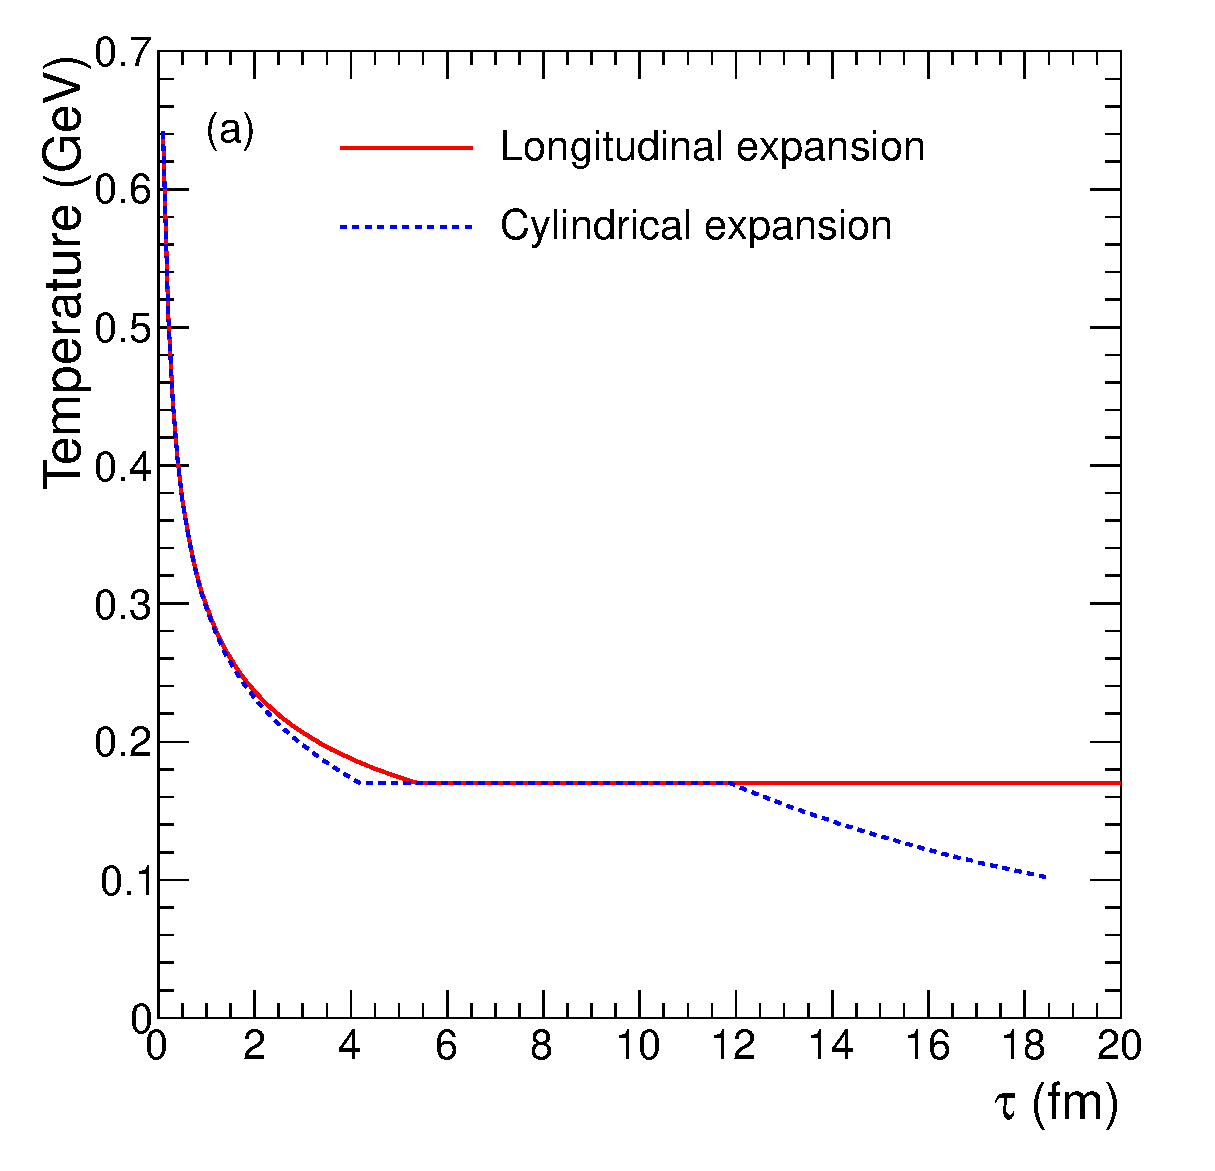
\includegraphics[width=0.49\textwidth]{Fig1a_TauVsTemp.eps}
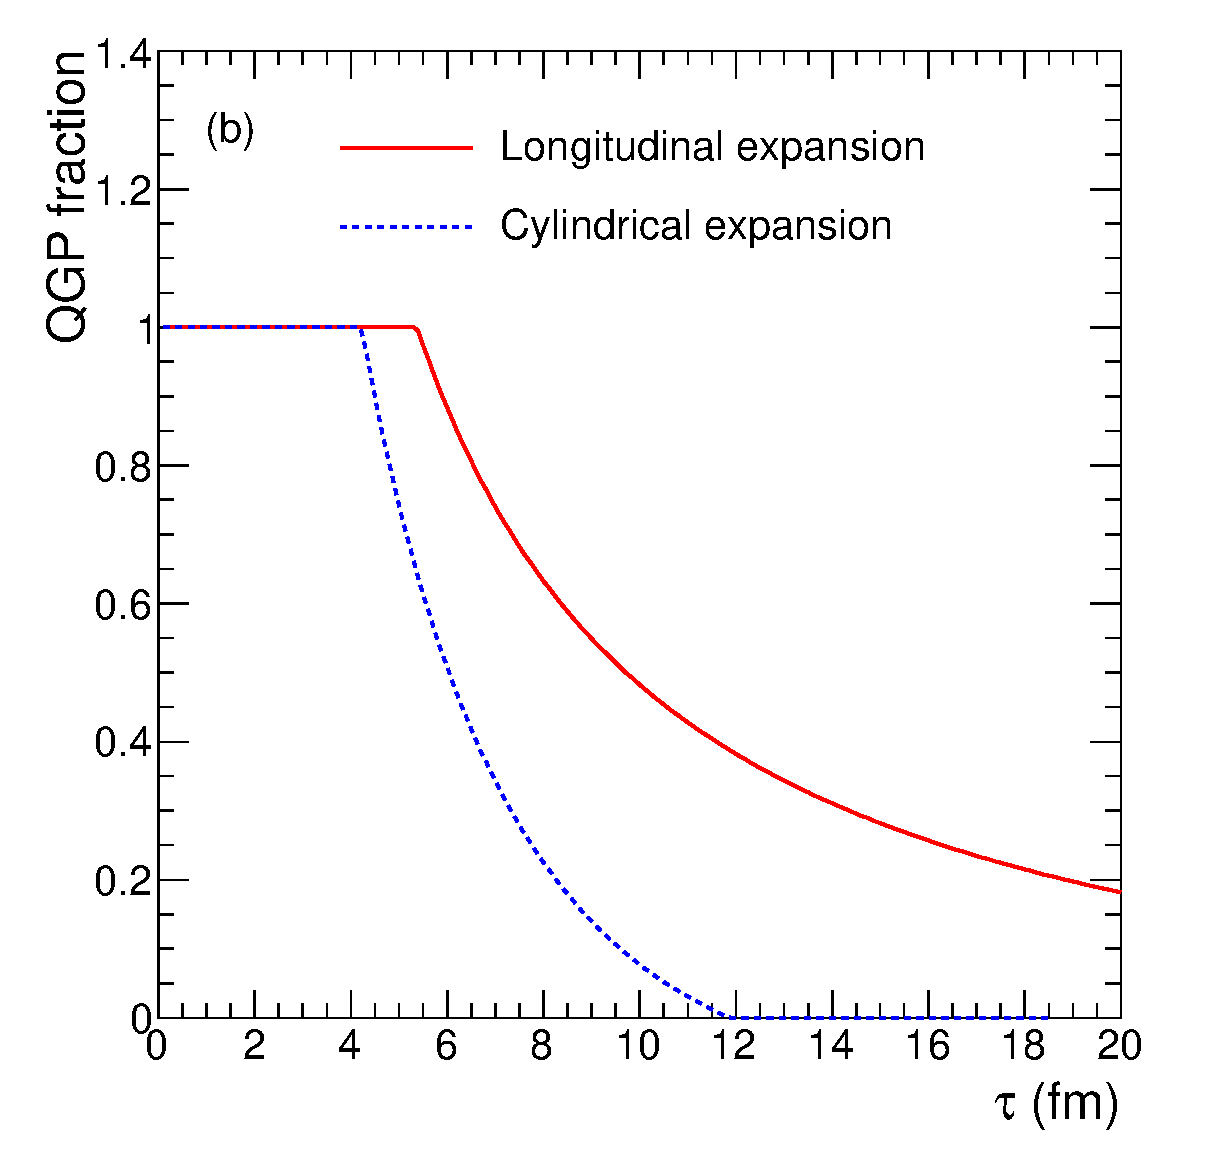
\includegraphics[width=0.49\textwidth]{Fig1b_TauVsFQGP.eps}
\caption{(Color online) (a) Temperature and (b) QGP fraction in the system as a function of proper 
time in case of most central (0-5$\%$) collisions for longitudinal and cylindrical expansions.}
\label{fig:TauVsTemp}
\end{figure}

%%%%%%%%%%%%%%%%%%%%%%%%%%%%%%%%%%%%%%%%%%%%%%%%%%%%%%%%%%%%%%%%%%%%%%%%%%%%%%%%%%%%%%%%%%%%%%%%%




\begin{table}
\caption[]{Quarkonia properties as predicted by non-relativistic potential model using 
``Cornell'' potential \cite{colorSatz}.}
\label{Tab:QuarkoniaProperties}
\begin{tabular}{l|l|l|l|l|l|l|l|l} 
\hline   
\hline
    &$\Jpsi$  &$\chi_c$  &$\psi(2S)$ &$\Upsilon(1S)$ &$\chi_b(1P)$ &$\Upsilon(2S)$ &$\chi_b(2P)$ &$\Upsilon(3S)$ \\ 
\hline 
Mass [GeV/$c^2$]                      &3.10     &3.53  &3.68  &9.46  &9.99  &10.02  &10.26   &10.36 \\
Binding Energy [GeV]                  &0.64     &0.20  &0.05  &1.10  &0.67  &0.54   &0.31    &0.20 \\
%Radius [fm]                           &0.25     &0.36  &0.45  &0.14  &0.22  &0.28   &0.34    &0.39 \\
%Formation time $\tau_{\rm Form}$ [fm]    &0.89     &2.0   &1.5   &0.76  &2.6   &1.9    &2.6      &2.4 \\
\hline
\hline
\end{tabular}
\end{table}


\subsection{Dissociation Rate}
   In colour dipole approximation the gluon dissociation cross section as function of gluon energy $q^0$
in the J$/\psi$ rest frame is given by \cite{BhanotPeskin}
\begin{equation}
\sigma_{D}(q^{0}) = 4\pi\,\left(\frac{8}{3}\right)^3\,\frac{1}{m_c^{3/2}}\,\epsilon_0^3 \frac{ (q^0-\epsilon_0)^{3/2}}{(q^0)^5},
\end{equation}
where $\epsilon_0$ is the $\Jpsi$ binding energy and $m_c$ is the charm quark mass.
The values of $\epsilon_0$ for different quarkonia states are given in Table~\ref{Tab:QuarkoniaProperties}.
 Figure \ref{fig:SigmaDQ0} shows the gluon dissociation cross section ($\sigma_{D}(q^{0})$) of $\Jpsi$ and $\Upsilon(1S)$
as a function of gluon energy. 
 The dissociation cross section is zero when gluon energy is less than the binding energy
of the $\Jpsi$. It increases with gluon energy and reaches  maximum at 1.2 (1.5) GeV for 
$\Jpsi\,(\Upsilon)$. At higher gluon energy gluons the interaction probability decreases.
$q^0$ is related to centre of mass energy $s$, of $\Jpsi$-gluon system as
\begin{eqnarray}
 q^{0} = \frac{s-M_{\Jpsi}^{2}}{2\,M_{\Jpsi}},
\end{eqnarray}  
  Using this relation $\sigma_{D}(q^0(s))$ can be obtained which we write as $\sigma_{D}(s)$.
The centre of mass energy square $s$, of $\Jpsi$-gluon system can be written as
$s=m_{\Jpsi}^{2} + 2E_{\Jpsi}E_{g}(1-{\rm cos\theta})$
here $E_g\,(E_{\Jpsi})$ is energy of gluon ($\Jpsi$) and $\theta$ is angle between them.
 
 We can calculate dissociation rate by folding the dissociation cross-section on thermal gluon 
distribution $f_{g}(p)$ as   
\begin{eqnarray}
\lambda_{D} \rho_{g}  & = & \langle \sigma v_{\rm rel} \rangle \,\rho_{g}  = 
      \frac{\lambda_g}{(2\pi)^{3}} \int d^{3}p \, f_{g}(p) v_{\rm rel} \, \sigma_{D}(s)   \nonumber \\ 
& = &\frac{\lambda_g}{(2\pi)^{3}} \int  2\pi p^{2} dp f_{g}(p) \int \sigma_{D}(s) v_{\rm rel}(s) d({\rm cos\theta})  
\end{eqnarray}
 The relative velocity $v_{\rm rel}$ between the $\Jpsi$ and gluon can be given by
\begin{eqnarray}
 v_{\rm rel}  = {s- M_{\Jpsi}^{2} \over 2E_{\Jpsi}E_{g}}  
\label{eq7}
\end{eqnarray}

 Figure \ref{fig:DRateVsTempAndPt} shows variation of gluon dissociation rate for $\Jpsi$ as a 
funcion of medium temperature and $\Jpsi$ transverse momentum. Dissociation rate increases with temperature because 
increase in gluon density. Dissociation is maximum if we consider $\Jpsi$ at rest and decreases 
with transverse momentum of $\Jpsi$.


\begin{figure}
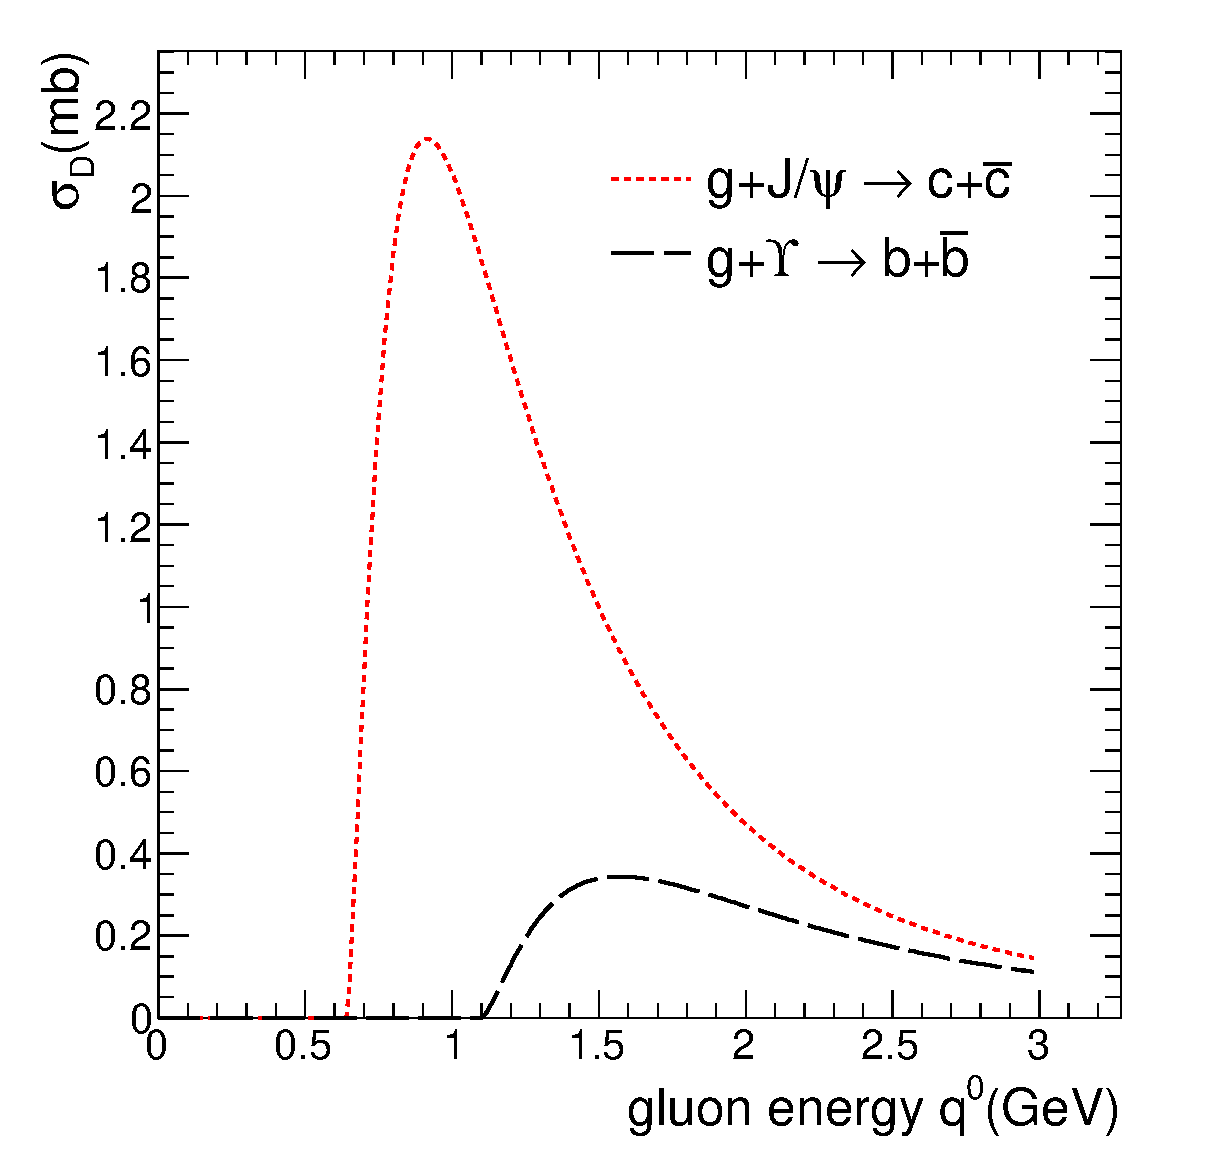
\includegraphics[width=0.60\textwidth]{Fig2_SigmaDq0.eps}
\caption{Gluon dissociation cross-section of quarkonia as a function of gluon energy ($q^{0}$) in
quarkonia rest frame.}
\label{fig:SigmaDQ0}
\end{figure}

\begin{figure}
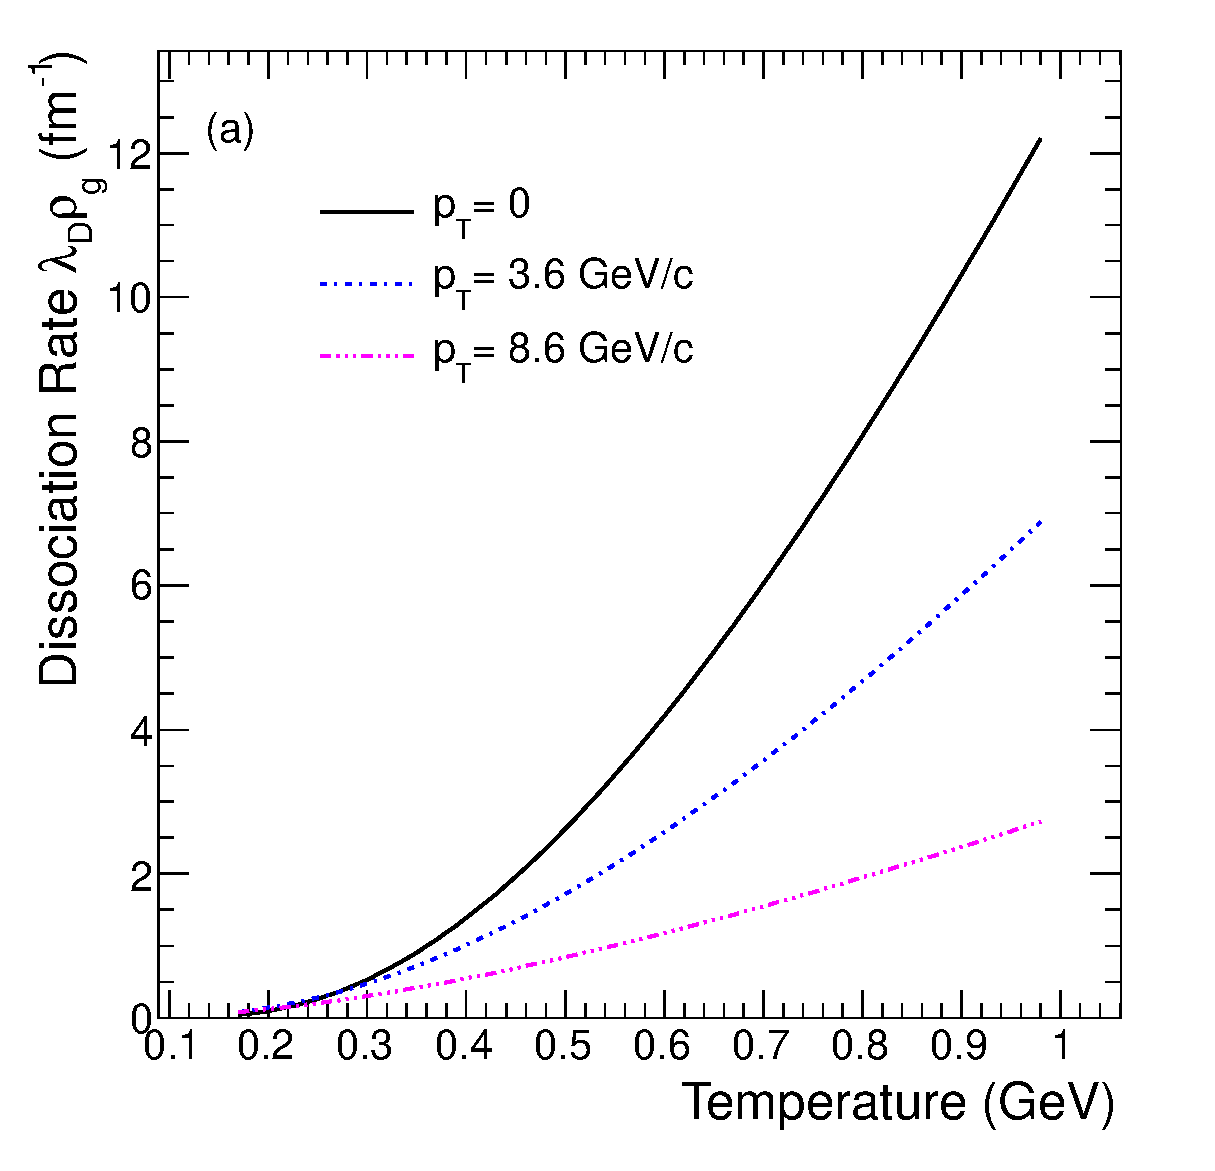
\includegraphics[width=0.49\textwidth]{Fig3a_DRateVsT.eps}
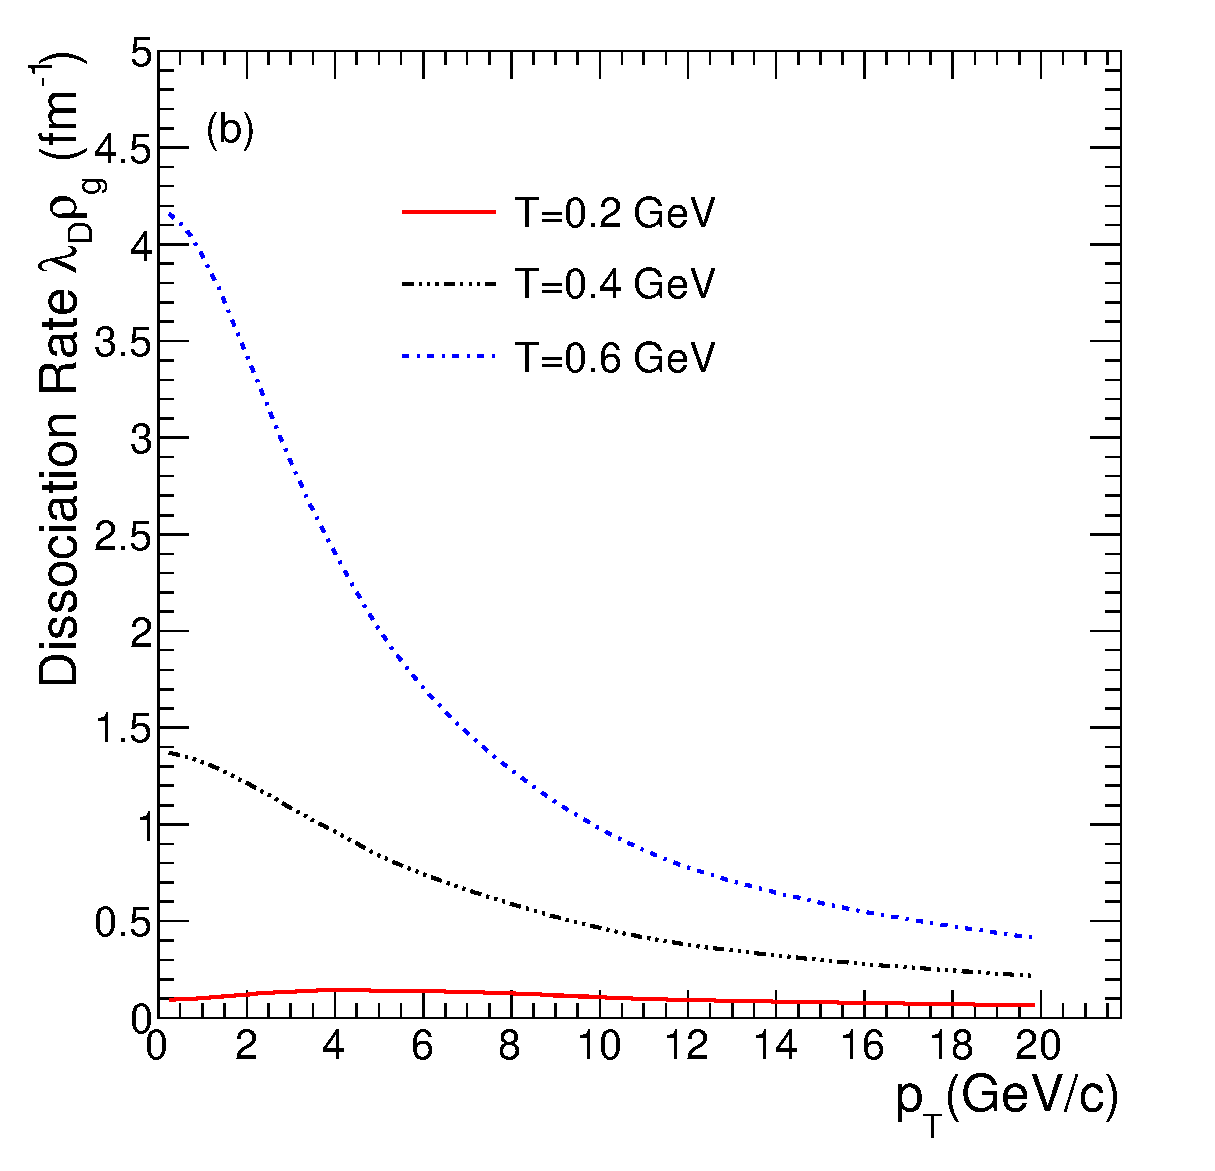
\includegraphics[width=0.49\textwidth]{Fig3b_DRateVsPt.eps}
\caption{(Color online) Gluon dissociation rate of $\Jpsi$ as a function of a) temperature and  b) transverse momentum.}
\label{fig:DRateVsTempAndPt}
\end{figure}



%
%and $q^0$ the gluon energy in the $J/ \psi$ rest frame is related to centre of mass 
%energy of $\Jpsi$-gluon system as
%\begin{eqnarray}
% q^{0} = \frac{s-M_{\Jpsi}^{2}}{2\,M_{\Jpsi}},
%\end{eqnarray}

%%%%%%%%%%%%%%%%%%%%%%%%%%%%%%%%%%%%%%%%%%%%%%%%%%%%%%%%%%%%%%%%%%%%
%%%%%%%%%%%%%%%%%%%%%%%%%%%%%%%%%%%%%%%%%%%%%%%%%%%%%%%%%%%%%%%%%%
%`If we consider that the $J/ \psi$ moves in the transverse direction with a four-velocity
%$u=(M_T, \vec{P_T}, 0)/M_{\Jpsi}$, where $M_T=\sqrt{p_T^2+M^2_{J/ \psi}}$ is defined as the $\Jpsi$'s
%transverse mass. 
%A gluon with a four-momentum $k=(k^0,\vec{k})$
%in the rest frame of the parton gas has an energy $q^0=k\cdot u$
%in the rest frame of the $\Jpsi$ given by
%\begin{eqnarray}
% q^{0} &= &\frac{k^{0}\,m_{T} + \vec{k} \cdot \vec{p_{T}}}{M_{\Jpsi}}, \nonumber \\
%       &= &\frac{s-M_{\Jpsi}^{2}}{2\,M_{\Jpsi}},
%\end{eqnarray}
%The dissociation rate is given by 
%\begin{eqnarray}
%\lambda_D = \langle v_{\rm rel} \sigma_{D} (k \cdot u)\rangle_k &= &\frac{\int d^3k v_{\rm rel} \sigma_{D} (k \cdot u) f(k^0,T)}{\int d^3k f(k^0,T)},
% \label{eq5}
%\end{eqnarray}
%where the gluon distribution in the rest frame of the parton gas is
%\begin{equation}
%  f(k^0,T)=\frac{\lambda_g(=16)}{e^{k^0/T}-1} \label{eq6}.
%\end{equation}
%The relative velocity $v_{\rm rel}$ between the $\Jpsi$ and a gluon is
%\begin{eqnarray}
% v_{\rm rel}  =  \frac{P_{\Jpsi}\cdot k}{k^0M_T} \,\,
%              =  1-\frac{\vec{k}\cdot\vec{P}_T}{k^0M_T} \,\,
%              =  {s- M_{\Jpsi} \over 2E_1E_2}  
%\label{eq7}
%\end{eqnarray}
%Changing the variable to the gluon momentum, $q=(q^0,\vec{q})$, in
%the rest frame of the $\Jpsi$, and writing $\rho_g = \int d^3k f(k^0,T)$, 
%the Eq.~(\ref{eq5}) can be rewritten as
%\begin{eqnarray}
%\lambda_D \rho_g  =  \int d^3q \frac{M_{\Jpsi}}{m_T}\sigma_{D}(q^0) f(k^0,T).
%\label{eq8}
%\end{eqnarray}
%Using $ k^0=(q^0M_T+\vec{q}\cdot\vec{P}_T)/M_{\Jpsi}$ in Eq.~\ref{eq8} and solving
%\begin{eqnarray} 
%\lambda_D\,\rho_g &= &\frac{M_{\Jpsi}}{m_T} \int d^3q \, \sigma_{D}(q^0) \frac{\lambda_{g}} {  e^{ \frac{q^0m_{T}}{M_{\Jpsi}T}} e^{ \frac{ \vec{q}\cdot \vec{p_{T} } }{ M_{\Jpsi}T }  } -1}  \nonumber \\
%%&= &\frac{\lambda_{g}}{2\pi^3} \frac{M_{\Jpsi}}{m_T} \int d^3q \, \sigma_{D}(q^0)   \sum_{n=1}^{\infty}  e^{ \frac{-n\,q^0 m_{T}}{M_{\Jpsi}T}} e^{  \frac{-n\,\vec{q}\cdot \vec{p_{T}}}{M_{\Jpsi}T}}  \nonumber \\
%%&= &\frac{\lambda_{g}}{2\pi^3} \frac{M_{\Jpsi}}{m_T}  \sum_{n=1}^{\infty} 2\pi  \int (q^0)^2 dq^0 \, \sigma_{D}(q^0)\,e^{ \frac{-n\,q^0m_{T}}{M_{\Jpsi}T}}  \int_{1}^{-1} e^{  \frac{-n\,q^0\,p_{T} cos\theta}{M_{\Jpsi}T}} d(cos\theta) \nonumber \\
%%&= &\frac{\lambda_{g}}{2\pi^3} \frac{M_{\Jpsi}}{m_T} \sum_{n=1}^{\infty} 2\pi  \int (q^0)^2 dq^0 \, \sigma_{D}(q^0)\,e^{ \frac{-n\,q^0 m_{T}}{M_{\Jpsi}T}} 
%%    \left[ e^{-\frac{nq^0 p_T}{M_{\Jpsi}T}} - e^{\frac{nq^0 p_T}{M_{\Jpsi}T}} \right]\,\frac{M_{\Jpsi}T}{nq^0 p_T}  \nonumber \\
%&= &\frac{\lambda_{g}}{2\pi^3} \frac{M_{\Jpsi}^2}{m_T} 2\pi \sum_{n=1}^{\infty} \frac{T}{n} \int_{\epsilon_0}^{\infty} q^0 dq^0 \, \sigma_{D}(q^0)  
%     \,e^{ \frac{-n\,q^0 m_{T}}{M_{\Jpsi}T}} 
%     \frac{1}{p_T} \left[e^{\frac{n q^0 p_T}{M_{\Jpsi}T}} - e^{- \frac{n q^0 p_T}{M_{\Jpsi}T}}\right] \\ \nonumber
%\label{dissrate}
%\end{eqnarray}

%%%%%%%%%%%%%%%%%%%%%%%%%%%%%%%%%%%%%%%%%%%%%%%%%%%%%%%%%%%%%%%%%%%%
%%%%%%%%%%%%%%%%%%%%%%%%%%%%%%%%%%%%%%%%%%%%%%%%%%%%%%%%%%%%%%%%%%%%
% The special case of Eq.~(\ref{dissrate}) for J/$\psi \,p_T = 0$ is
%\begin{eqnarray} 
%  \frac{1}{p_T} \left[e^{\frac{n q^0 p_T}{M_{\Jpsi}T}} - e^{- \frac{n q^0 p_T}{M_{\Jpsi}T}}\right] = {2nq^0\over M_{\Jpsi}T}.
%\label{case}
%\end{eqnarray}
%Using this we get 
%\begin{eqnarray} 
% \lambda_D\,\rho_g &= &  4\pi \int (q^0)^2\,dq^0 \, \sigma_{D}(q^0) \frac{\lambda_{g}} {e^{\frac{q^0}{T}} -1}
%\end{eqnarray}

%%%%%%%%%%%%%%%%%%%%%%%%%%%%%%%%%%%%%%%%%%%%%%%%%%%%%%%%%%%%%%%%%%%%%%%%%%%%%%%%%%%%
\subsection{Formation Rate}
  We can calculate formation cross section from dissociation cross section using detailed balance 
relation \cite{Thews,THEWF} as
\begin{equation}
\sigma_{F} = \frac{48}{30}\,\sigma_{D}(q^0)\frac{(s-M_{\Jpsi})^{2}}{s(s-4m_{c}^{2})}.
\end{equation}
The formation rate can be written as
\begin{equation}
\lambda_{F} = \langle \sigma_{F} \,\, v_{\rm rel} \rangle = \frac{\int \sigma_{F}(s)\, v_{\rm rel}\,f_{c}(p_1)\, f_{\bar{c}} (p_2) \,d^{3}p_1 \,d^{3}p_2 \, \delta^{3}(\vec{p}-(\vec{p_1}+\vec{p_2}))} 
       {\int \,f_{c}(p_1)\,d^{3}p_1 \,\, \int f_{\bar{c}} (p_2)\,d^{3}p_2}.
\end{equation}
Here $f_{c/\bar{c}}(p)$ are taken as thermal distribution function of  $c/\bar{c}$.
$v_{\rm rel}$ is relative velocity between c $\bar{c}$ quark pair and is given by
\begin{eqnarray}
v_{\rm rel} &=& {\sqrt{(p_{1}.p_{2})^{2} - m_c^{4} } \over E_{1} \, E_{2}} \nonumber \\
            &=& \frac{\sqrt{s(s-4m_{Q}^{2})}}{2E_1E_2}.
\end{eqnarray}
 Here $p_1 = (E_1,\vec{p_{1}})$, $p_{2} = (E_{2},\vec{p_{2}})$ are four vectors of charm and anti-charm 
quarks respectively. The centre of mass energy square of c$\bar{c}$ system is 
 $s =  2\,m_c^{2} + 2 E_1E_2 - 2 |\vec{p_1}||\vec{p_2}|cos\theta$.

Figure \ref{fig:ForRateVsTempAndPt} shows variation of formation rate as a funcion of medium temperature
and transverse momentum. The $\Jpsi$ generated from recombination of uncorrelated heavy quark pairs will have 
softer $p_{T}$ distributions than that of $\Jpsi$ coming from initial hard scattering and thus 
effect of recombination will be important only at low $p_T$.

\begin{figure}
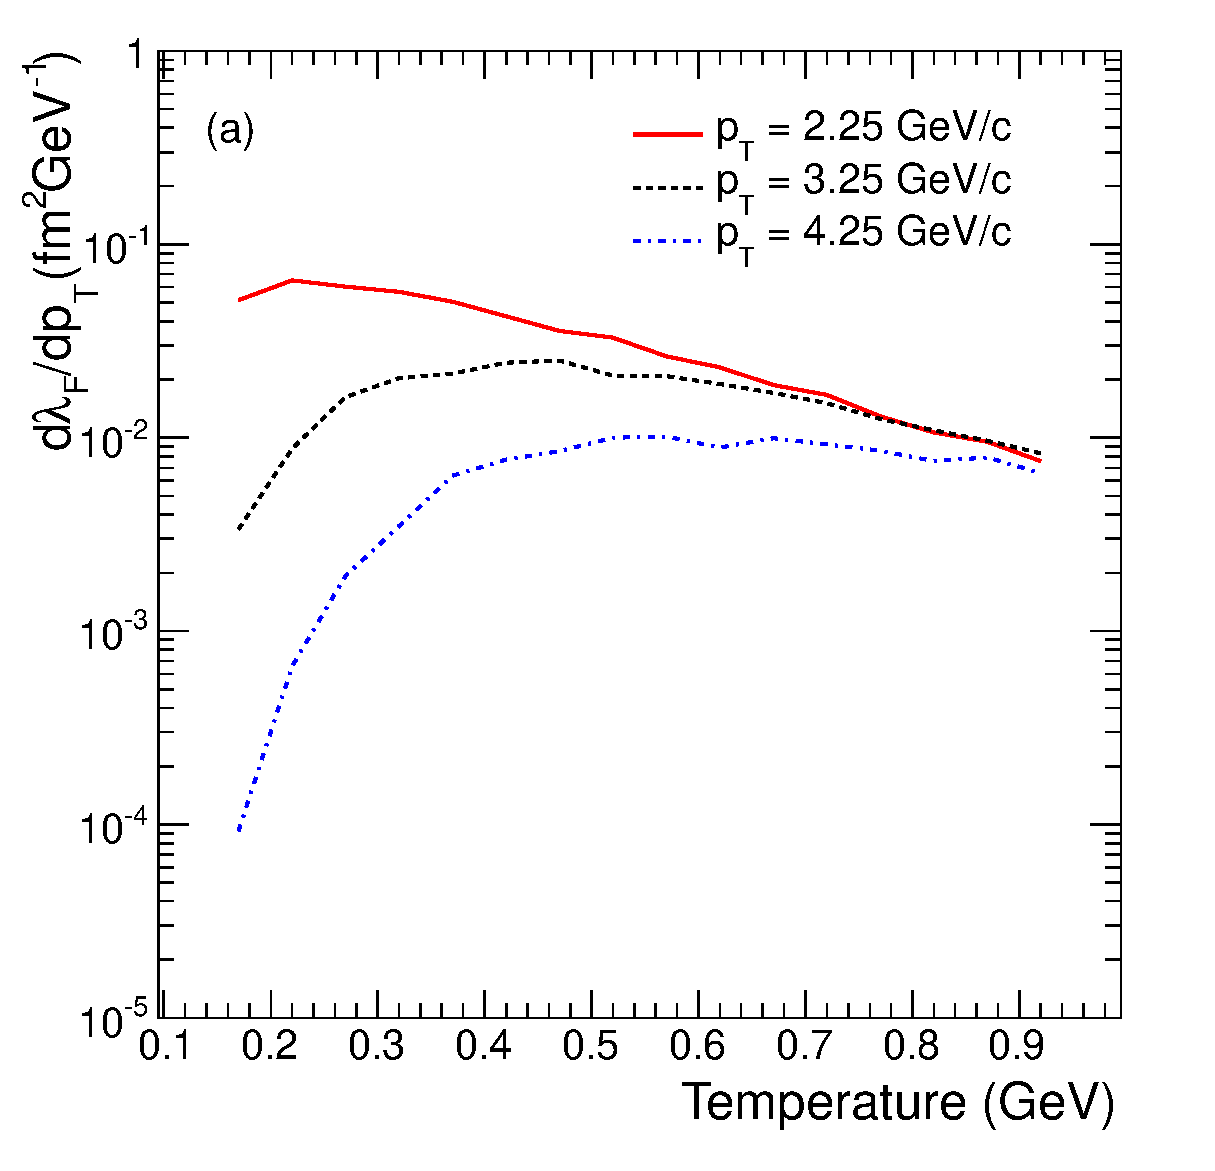
\includegraphics[width=0.49\textwidth]{Fig4a_FRateVsT.eps}
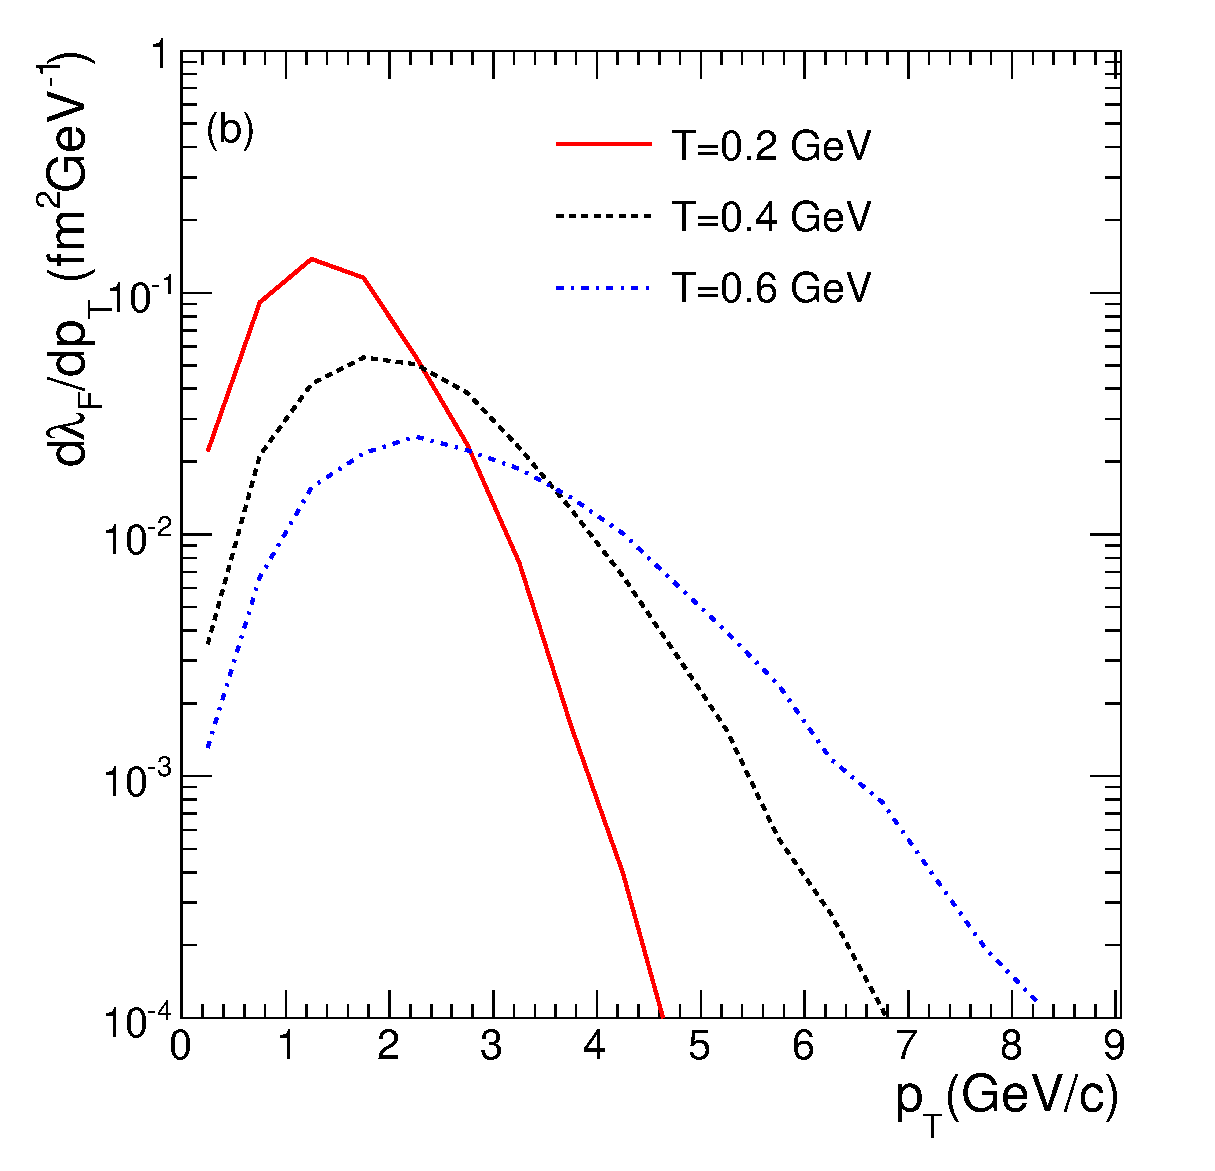
\includegraphics[width=0.49\textwidth]{Fig4b_FRateVsPt.eps}
\caption{(Color online) Formation rate as a function of (a) temperature and (b) transverse momentum.}
\label{fig:ForRateVsTempAndPt}
\end{figure}

The formation and dissociation rates are shown for $\Jpsi$, we use same formalism to calculate
these rates for $\Upsilon$ also.


\begin{figure}
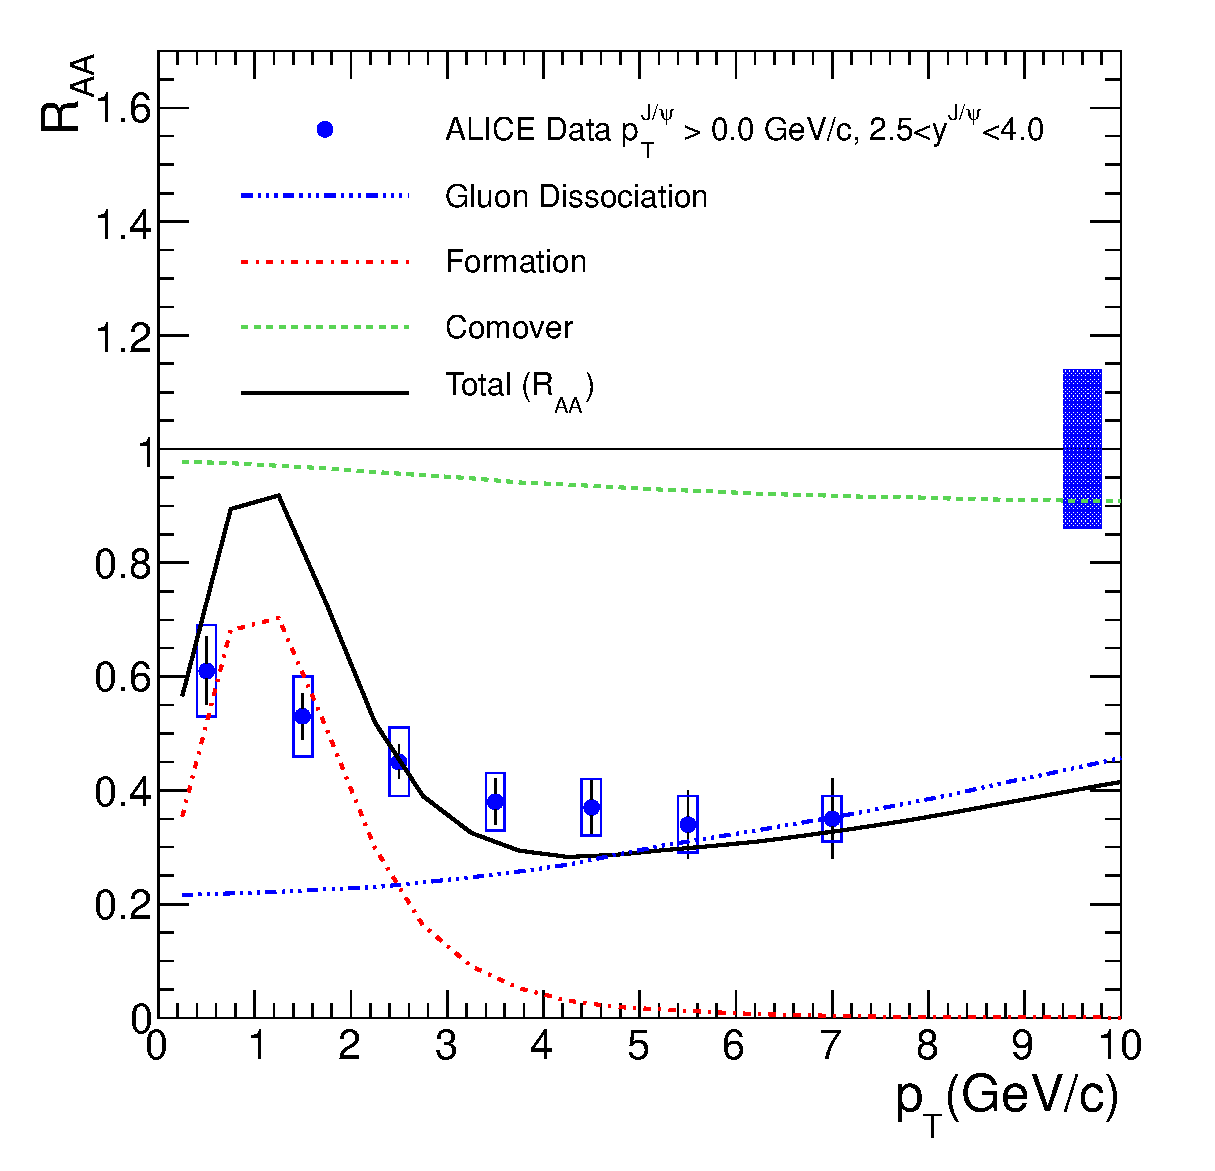
\includegraphics[width=0.49\textwidth]{ALICE_RAAPt.eps}
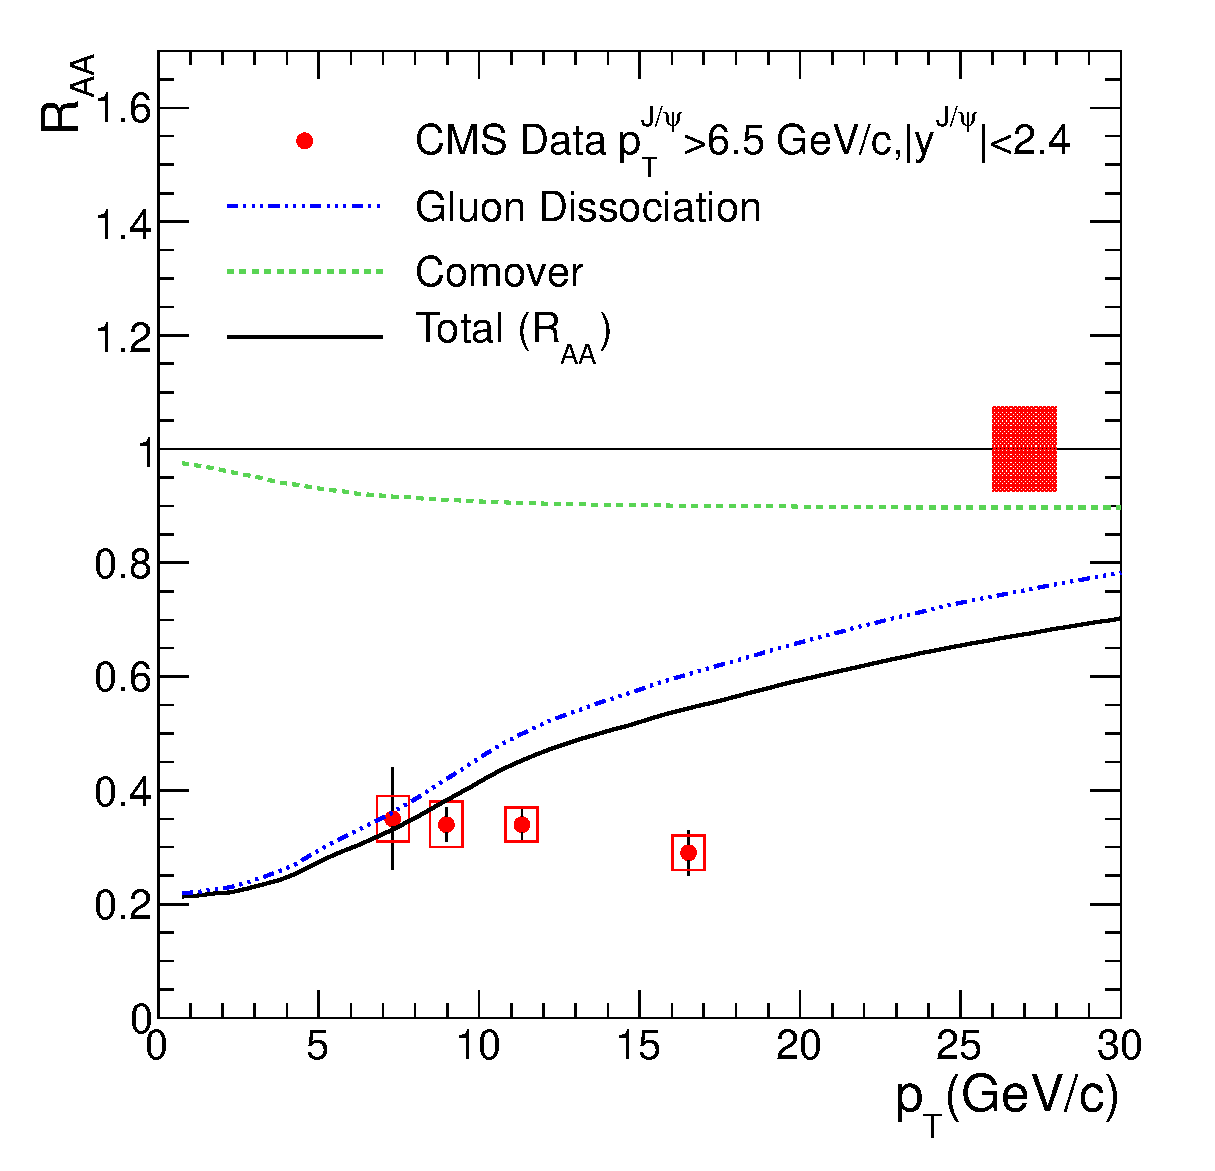
\includegraphics[width=0.49\textwidth]{CMS_RAAPt.eps}
\caption{(Color online) Calculated nuclear modification factor (R$_{AA}$) as a function of $\Jpsi$ transverse momentum. Calculations are
compared with ALICE and CMS measurements.}
\label{fig:JPsiRaaVsPt}
\end{figure}


%%%%%%%%%%%%%%%%%%%%%%%%%%%%%%%%%%%%%%%%%%%%%%%%%%%%%%%%%%%%%%%%%%%%%%%%%%%%%%%%%%%%%%
%\section{Formation of quarkonia  by statistical hadronization model}\label{SHM}
% The heavy quark production at LHC is substantial which may lead to incoherent 
%recombination of uncorrelated pairs of heavy quarks and anti quarks which result 
%from multiple pair production. In statistical approach \cite{MUNZI} the number of 
%$\Jpsi$ regenrated is given by 
%\begin{eqnarray}
%N_{\Jpsi}  &= &4 {n_{ch} n_{\Jpsi} \over n_{\rm open}^2}  {N_{c\bar c}^2 \over N_{ch} }\\
%          &= &\frac{N_{c\overline{c}}^{2}}{V}\frac{4n_{\Jpsi}}{n_{open}^{2}}.
%\end{eqnarray}
%where $n_i$'s are the thermal densities, $N_{c\bar c}$ is the number of charm pairs produced 
%and $N_{ch}$ is the number of total charged particle produced. 
%The freeze out parameters are $T=170$ MeV and $\mu_B = 0$. For
%$dN_{ch}/dy = 1600$ \cite{MULT} and $dN_{c \bar c} /dy = 14.0$, we obtain $dN_{\Jpsi} /dy = 0.0092$.


\begin{figure}
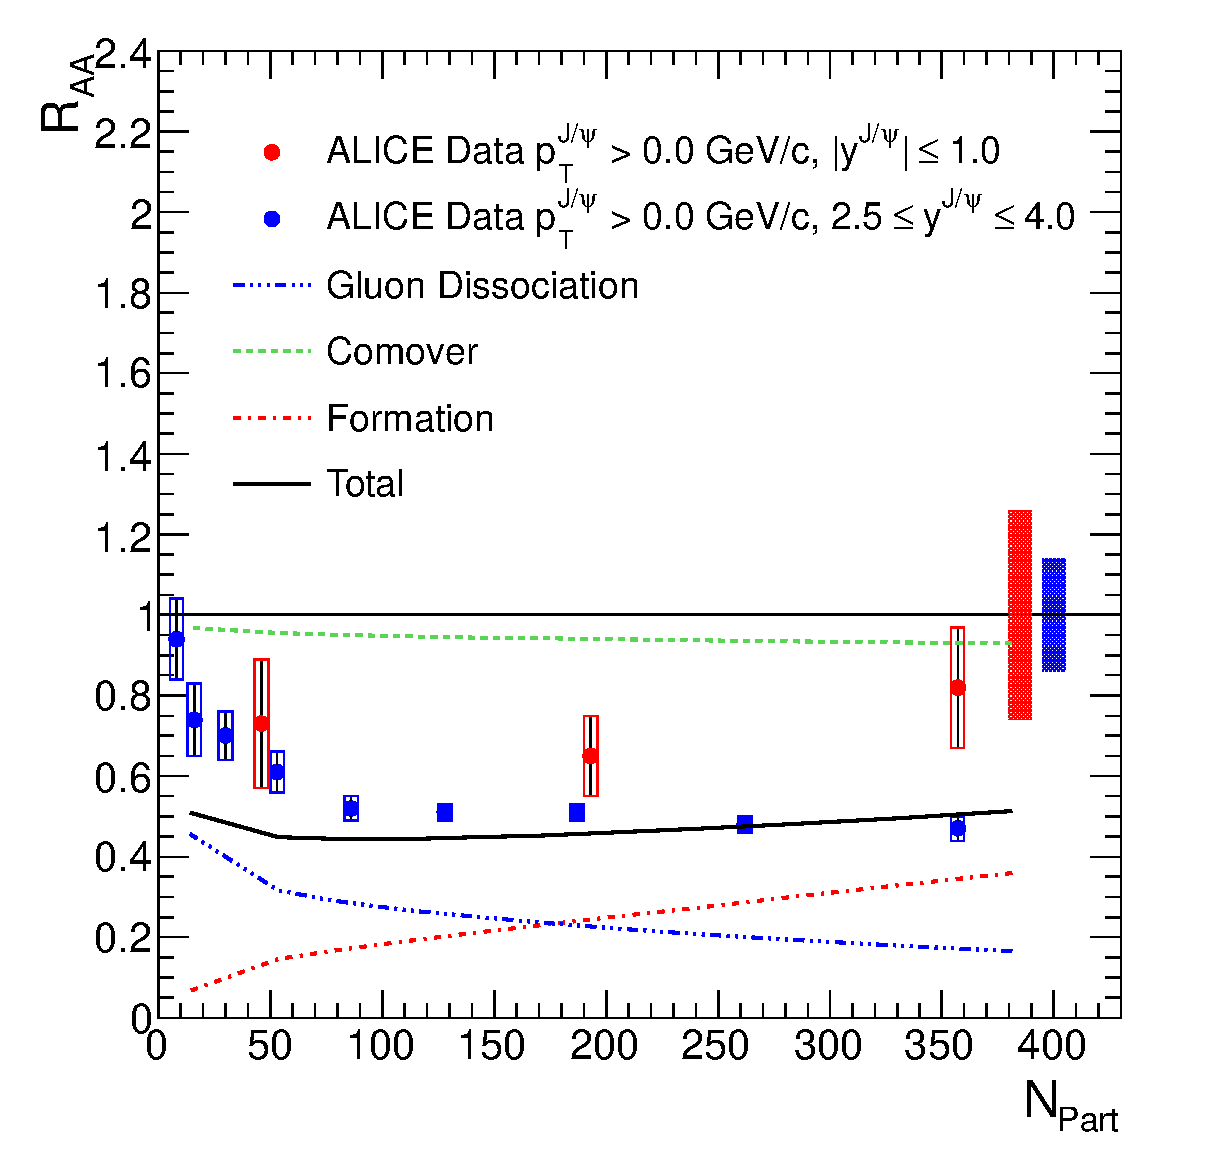
\includegraphics[width=0.49\textwidth]{ALICE_RAA.eps}
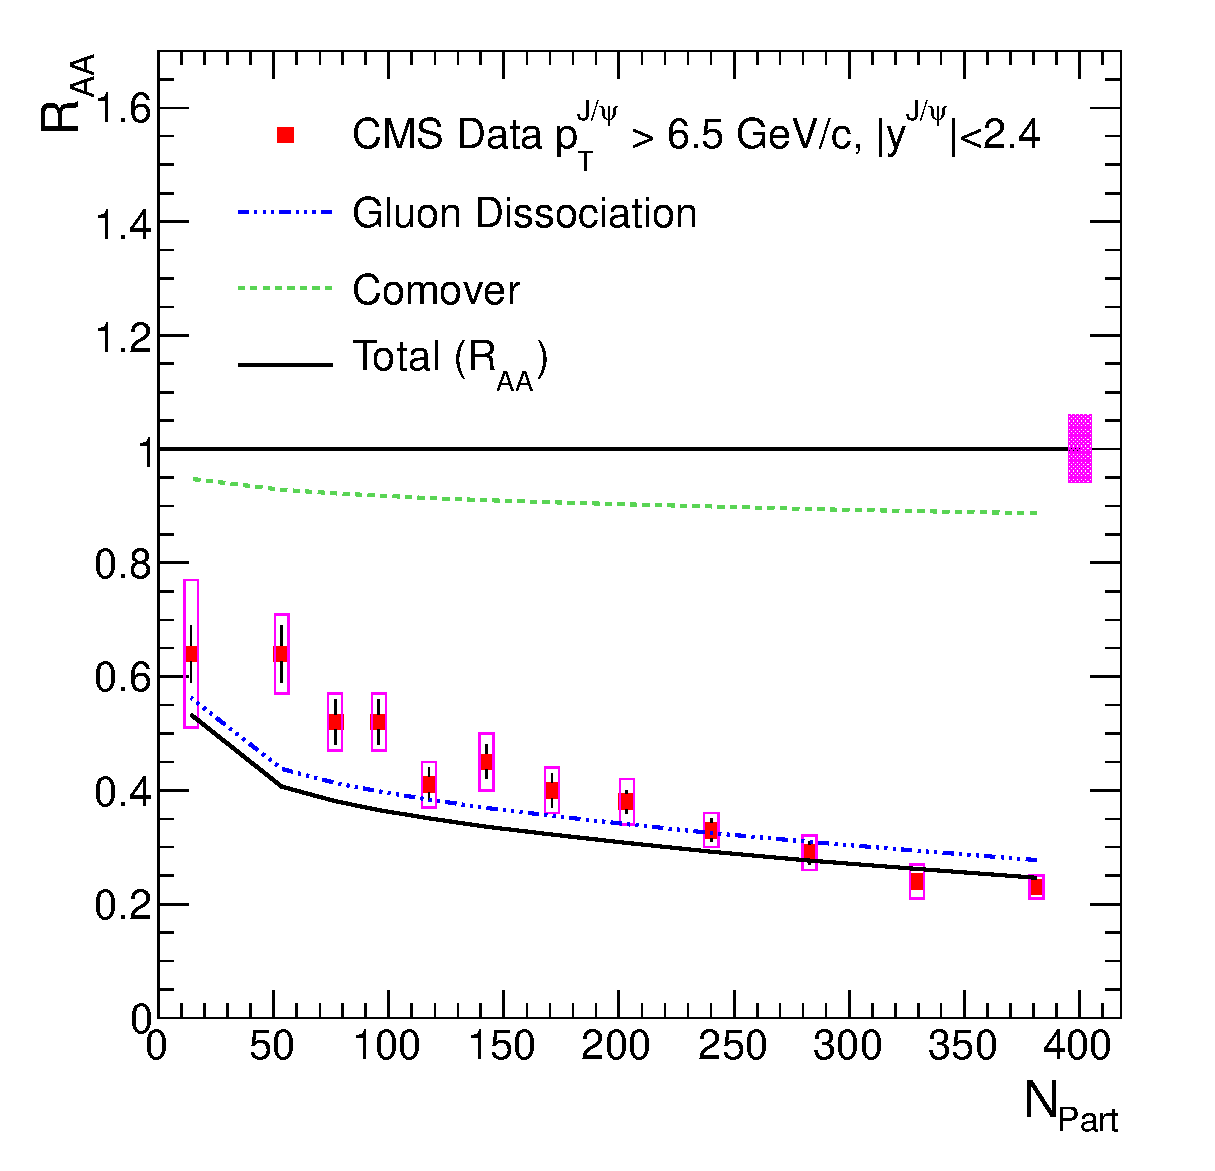
\includegraphics[width=0.49\textwidth]{CMS_RAA_JPsi.eps}
%\caption{(Color online) Calculated nuclear modification factor (R$_{AA}$) compared with ALICE and CMS measurements at LHC. No regeneration is 
%considered for high p$_{T}$ CMS data. We assume similar cold nuclear matter effects for both ALICE and CMS rapidity ranges.}
\caption{(Color online) Calculated nuclear modification factor (R$_{AA}$) compared with ALICE and CMS measurements at LHC. No regeneration is 
considered for high p$_{T}$ CMS data. We assume similar cold nuclear matter effects for both ALICE and CMS rapidity ranges.}
\label{fig:JPsiRaa}
\end{figure}


\begin{figure}
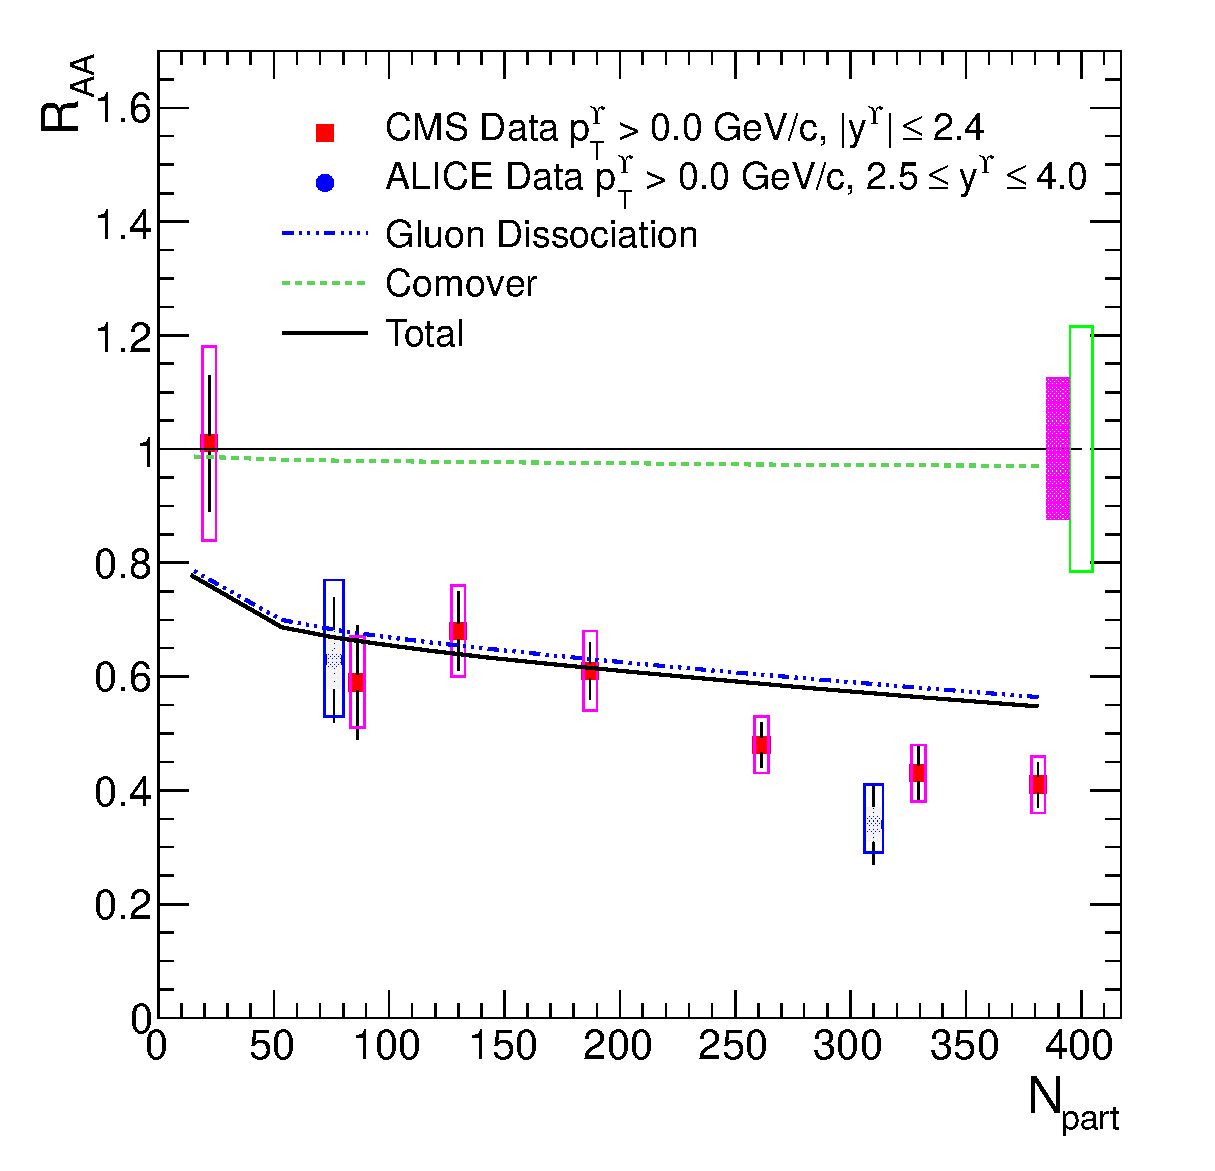
\includegraphics[width=0.49\textwidth]{CMS_RAA_Upsilon1S.eps}
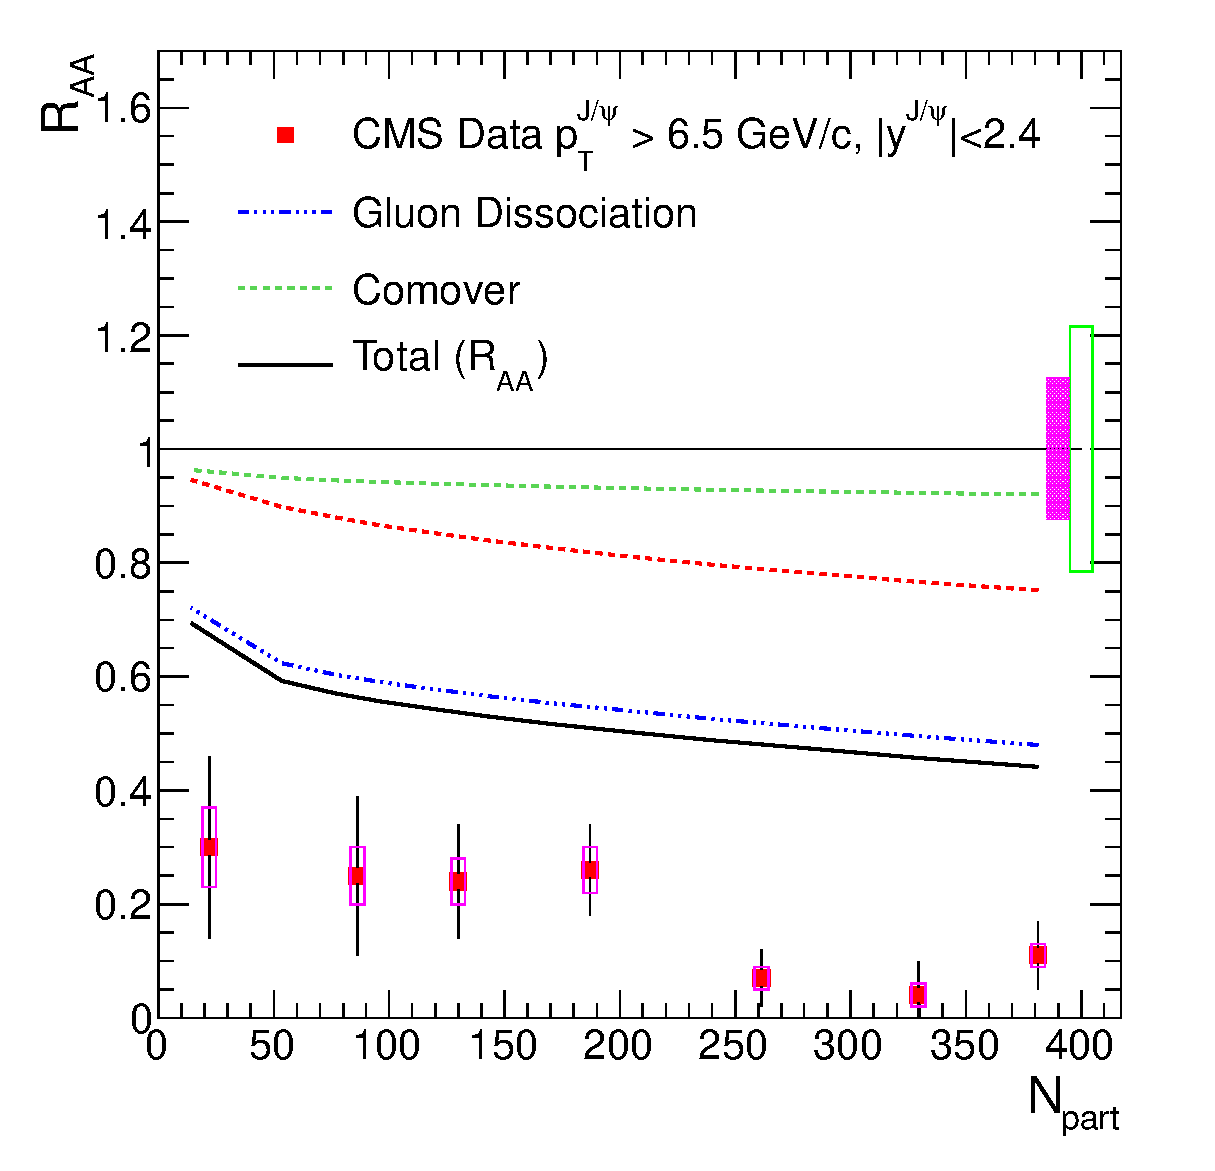
\includegraphics[width=0.49\textwidth]{CMS_RAA_Upsilon2S.eps}
%\caption{(Color online) Calculated nuclear modification factor (R$_{AA}$) compared with CMS $\Upsilon$(1S) and $\Upsilon$(2S) measurements.
%We assume small cold nuclear matter suppression than J$\psi$ and no regeneration due to small production cross section of beauty quark as shown in Table~\ref{NLOcros}.}
\caption{(Color online) Calculated nuclear modification factor (R$_{AA}$) compared with CMS $\Upsilon$(1S) and $\Upsilon$(2S) measurements.
We assume small cold nuclear matter suppression than J$\psi$ and no regeneration due to small production cross section of beauty quark as shown in Table~\ref{NLOcros}.}
\label{fig:UpsilonRaa}
\end{figure}

%%%%%%%%%%%%%%%%%%%%%%%%%%%%%%%%%%%%%%%%%%%%%%%%%%%%%%%%%%%%%%%%%%%%%%%%%%%%%%%%%%%%%%%%
\section{Cold matter effects}
%The quarkonia can be suppressed due to cold matter effects such as shadowing and due to hadronic
%and comover interaction. For simplicity we approximate the combination of all CNM effects 
%by a suppression factor \cite{Rapp1,Rapp2},
%\begin{equation}
%  S_{Nucl}=\exp[-\rho_{N}\sigma_{abs}L(b)]
%  \label{CNMF}
%\end{equation}
%with an effective nuclear absorption cross section, $\sigma_{abs}$.
%We take absorption cross section, $\sigma_{abs}$ = 1.5 mb (1.5 mb) for
%$\Jpsi$($\Upsilon$). The other parameters in Eq. \ref{CNMF} are the nuclear density,
%$\rho_N$=0.14 fm$^{-3}$, and the impact-parameter dependent path length, L(b), evaluated 
%with a Glauber model \cite{GM_PShukla} for the nuclear overlap.
The suppression of quarkonia by comoving pions can be calculated by folding the $\Jpsi$-pion
dissociation cross section over thermal pion distributions \cite{vogt2}. If we assume a constant dissociation 
cross section $\sigma_{I}$, the dissociation rate $\lambda_{D_{\pi}}$  can be written as
\begin{eqnarray}
\lambda_{D_{\pi}} \, \rho_{\pi} & = & \frac{g_\pi}{(2\pi)^{3}} \int d^{3}p f_{\pi}(p) v_{\rm rel} \sigma_{I}\\ \nonumber
                   & = &\frac{1}{(2\pi)^{3}} \int  2\pi p^{2} dp f_{\pi}(p) \int \sigma_{I} v_{\rm rel}(s) \Theta(s-4m_{D}^{2}) d(cos\theta) \\\nonumber
\end{eqnarray}
where is $f_{\pi}(p_{\pi},T)$ the thermal pion distribution and the  pion density $\rho_{\pi}$ is given by 
\begin{eqnarray}
\rho_\pi =\frac{g_\pi}{(2\pi)^{3}} \int d^3p \, f_{\pi}(p) 
\end{eqnarray}

The survival probability from pion collisions at freeze-out time $\tau_f$ is written as
\begin{equation}
S(p_T) = \exp \left( {-\int_{\tau_0}^{\tau_f} (1-f(\tau)) \lambda_{D_{\pi}}(T,p_T)\,\rho_{\pi}(T)\,d\tau} \right).
\end{equation}
The temperature $T(\tau)$ and the QGP fraction $f(\tau)$ evolve from initial time $\tau_0$ to freeze-out time
$\tau_f$ due to expansion of QGP.


\section{Results and discussion}
Figure~\ref{fig:JPsiRaaVsPt} shows comparison of our calculations with $\Jpsi$ Nuclear Modification Factor ($R_{AA}$) as a 
function of transeverse momentum measured by ALICE \cite{ALICEJPsi} and CMS \cite{CMSJPsi} experiments.
 Our model with gluon dissociation, $\Jpsi$ regenration and comover suppression describes the ALICE data very well. 
However only gluon dissociation is not enough to explain the $\Jpsi$ high $p_{T}$ data mesured by CMS experiment and
shown in Figure~\ref{fig:JPsiRaaVsPt} (b). We consider the contributions of recombined $\Jpsi$ only for low $p_{T}$ 
measurements made by ALICE detector as shown in Fig. \ref{fig:JPsiRaaVsPt} (a). We can see from this Figure 
that regenrated $\Jpsi$ have very soft $p_{T}$ distribution and do not contribute much after 4 GeV/c. 
So We do not consider effect of regenration for high $p_{T}$ measurement made by CMS detector as shown in 
Figure~\ref{fig:JPsiRaaVsPt} (b). 
Figure~\ref{fig:JPsiRaa} (a) shows comparison of our calculations with $\Jpsi$ 
Nuclear Modification Factor as a function of event centrality measured by ALICE \cite{ALICEJPsi}
experiment in forward and central rapidities. $R_{AA}$ is lower in forward rapidity region (most central collisions) 
in comparison to the mid rapidity region. It indicate persence of additional cold nucler matter effects in forward 
rapidity or stronger recombination in mid rapidity. Our calculations explain the data very well in both mid and
forward rapidity region.
Figure~\ref{fig:JPsiRaa} (b) shows high $p_{T}\,\Jpsi\,R_{AA}$ measured by CMS experiment \cite{CMSJPs}.
It shows large suppression with strong centrality dependence. Our calculations matches very nicely with 
measured $\Jpsi\,R_{AA}$. 
Figure~\ref{fig:UpsilonRaa} (a) shows centrality dependence of $\Upsilon(1S)$ nuclear modification factor
measured in mid rapidity by CMS experiment\cite{CMSUpsilon2} and in forward rapidity by ALICE experiment 
\cite{ALICEUpsilon}. Figure~\ref{fig:UpsilonRaa} (b) shows the transeverse momentum dependence of 
$\Upsilon$ nuclear modification factor measured by CMS experiment \cite{JCMS}. As production cross section of 
bottom quark is small even at LHC energies, we do not consider effect of recombination for $\Upsilon$ calculations.
Our calculations give good description of data.

%%%%%%%%%%%%%%%%%%%%%%%%%%%%%%%%%%%%%%%%%%%%%%%%%%%%%%%%%%%%%%%%%%%%%%%%%%%%%%%%%%%%%%%
\section{Summary}
 The $\Jpsi$ and $\Upsilon$ modification in medium are calculated and compared to the data
measured by CMS and ALICE.
  The $\Jpsi$ suppression is estimated using process of gluon dissociation in medium. The rate of regeneration 
has been obtained using principle of detailed balance and is compared with that obtained using statistical 
hadronization model. 
The nuclear modification factor as a function of centrality and transverse momentum has been calculated  
and compared to $\Jpsi$ and $\Upsilon$ nuclear modification factors measured in PbPb collisions 
at $\sqrt s_{NN}$ =  2.76 TeV.
  Our model with both, gluon dissociation and nuclear absorption describes the data very well although, 
slight difference in most central collisions may be due to reduction of binding energy of quarkonia with 
temperature and lowering of quark mass.



\noindent
\begin{thebibliography}{100}
\medskip

\bibitem{SATZ} T. Matsui and H. Satz, Phys. Lett. B{\bf 178}, 416 (1986).
	
\bibitem{Schukraft} J. Schukraft, arXiv:1311.1429 [hep-ex].

\bibitem{Kluberg:2009wc}  L.~Kluberg and H.~Satz, arXiv:0901.3831 [hep-ph].

\bibitem{Brambilla:2010cs}  N.~Brambilla, S.~Eidelman, B.~K.~Heltsley, R.~Vogt, G.~T.~Bodwin, 
  E.~Eichten, A.~D.~Frawley and A.~B.~Meyer {\it et al.},  Eur.\ Phys.\ J.\ C {\bf 71}, 1534 (2011); arXiv:1010.5827 [hep-ph].

\bibitem{Rapp:2008tf}  R.~Rapp, D.~Blaschke and P.~Crochet, Prog.\ Part.\ Nucl.\ Phys.\ {\bf 65}, 209 (2010); arXiv:0807.2470 [hep-ph].

\bibitem{Andronic_SH1} A. Andronic, P. Braun-Munzinger, K. Redlich, J. Stachel, Phys. Lett. B {\bf 571}, 36 (2003); nucl-th/0303036.

%\bibitem{BraunMunzinger:2009ih} P.~Braun-Munzinger and J.~Stachel, arXiv:0901.2500 [nucl-th].
 
\bibitem{QGP_Tc} B. Muller, J. Schukraft and B. Wyslouch, Ann. Rev. Nucl. Part. Sci. {\bf 62}, 361-386 (2012);arXiv:1202.3233 [hep-ex].

\bibitem{JCMS} S. Chatrchyan {\it et al.} (CMS Collaboration) J. High Energy Phys. {\bf 1205}, 63 (2012);arXiv:1201.5069 [nucl-ex].

\bibitem{CMSJPsi} Camelia Minrov (CMS Collaboration) Nucl. Phys. A {\bf 904}, 194 (2013).

\bibitem{STARjpsi} Zebo Tang (STAR Collaboration) J. Phys. G {\bf 38}, 124107 (2011);arXiv: 1107.0532 [nucl-ex].

\bibitem{ALICEJPsi} Enrico Scomparin (ALICE Collaboration) Nucl. Phys. A {\bf 904}, 202 (2013).

\bibitem{PHENIXJPsi} A. Adare {\it et al.} (PHENIX Collaboration) Phys. Rev. C {\bf 84}, 054912 (2011);arXiv:1103.6269.

\bibitem{ALICEJPsi} Abelev B. {et. al.} (ALICE Collaboration) arxiv:1311.0214 [nucl-ex].
%\bibitem{Abelev:2012rv} Abelev 2012.

\bibitem{CMSUpsilon1} S. Chatrchyan {\it et al.} (CMS Collaboration) Phys. Rev. Lett. {\bf 107}, 052302 (2011).

\bibitem{CMSUpsilon2} S. Chatrchyan {\it et al.} (CMS Collaboration), Phys. Rev. Lett. {\bf 109}, 222301 (2012). 

\bibitem{ALICEUpsilon} Plash Khan (ALICE Collaboration) arXiv:1310.2565 [hep-ex].


\bibitem{YSuppAbdShuk} A. Abdulasalam and P. Shukla, Int. J. Mod. Phys. {\bf A}, 28 (2013) 1350105; arXiv:1210.7584.

\bibitem{BhanotPeskin} G. Bhanot and M. E. Peskin Nucl. Phys. B {\bf 156}, 391 (1979).

\bibitem{Xu} X. M. Xu, D. Kharzeev, H. Satz, and X. N. Wang, Phys. Rev. C {\bf 53}, 3051 (1996); hep-ph/9511331.

\bibitem{Andronic_SH2} A. Andronic, P. Braun-Munzinger, K. Redlich, J. Stachel Nucl. Phys. A {\bf 905}, 535 (2013); arXiv:1210.7724 [hep-ph].

\bibitem{Grandchamp} L. Grandchamp and R. Rapp, Phys. Lett. B {\bf 523}, 60 (2001); hep-ph/0103124.

\bibitem{Thews} R. L. Thews, M. Schroedter, J. Rafelski, Phys. Rev. C {\bf 63}, 054905 (2001); hep-ph/0007323.

\bibitem{Vogt} R. Vogt, Phys. Rev. C{\bf 81}, 044903 (2010); arXiv:1003.3497.

\bibitem{Rapp1} X. Zhao and R. Rapp, Nucl. Phys. A{\bf 859}, 114 (2011); arXiv:1102.2194.
 
\bibitem{Rapp2} X. Zhao and R. Rapp, Phys. Rev. C{\bf 82}, 064905 (2010); arXiv:1008.5328.

\bibitem{CTEQ6} J.~Pumplin, D.~R.~Stump, J.~Huston, H.~L.~Lai, P.~M.~Nadolsky 
and W.~K.~Tung,  JHEP {\bf 0207}, 012 (2002) [arXiv:hep-ph/0201195];
  D.~Stump, J.~Huston, J.~Pumplin, W.~K.~Tung, H.~L.~Lai, S.~Kuhlmann  and J.~F.~Owens,
  JHEP {\bf 0310}, 046 (2003)  [arXiv:hep-ph/0303013].

\bibitem{EPS09} K. J. Eskola, H. Paukkunen and C. A. Salgado, JHEP{\bf 0904}, 065 (2009); arXiv:0902.4154.

\bibitem{CNV} M. Cacciari, P. Nason and R. Vogt, Phys. Rev. Lett.{\bf 95}, 122001 (2005).

\bibitem{MNR} M. L. Mangano, P. Nason, and G. Ridolfi, Nucl. Phys. B{\bf 373}, 295 (1992).

\bibitem{ContinuumVKShuk} V. Kumar, P. Shukla and R. Vogt, Phys. Rev. C{\bf 86}, 054907 (2012).

\bibitem{PbPbTotal} S. Chatrchyan {\it et al.} (CMS Collaboration) Phys. Rev. C {\bf 84}, 024906 (2011).

\bibitem{Pythia1} Torbjorn Sjostrand, Stephen Mrenna, Peter Z. Skands J. High Energy Phys. {\bf 0605}, 026 (2006). 

\bibitem{Pythia2} Torbjorn Sjostrand, Stephen Mrenna, Peter Z. Skands Comput.Phys.Commun. {\bf 178} 852-867 (2008).

\bibitem{MULT} K. Aamodt {\it et al.} (ALICE collaboration), Phys. Rev. Lett. {\bf 106}, 032301 (2011); arXiv:1012.1657 [nucl-ex].

\bibitem{colorSatz} F. Karsch, M. T. Mehr and H. Satz, Z. Phys. C {\bf 37}, 617 (1988).

\bibitem{THEWF} R.L. Thews and M.L. Mangano, arXiv:nucl-th/05050552 (2006).

\bibitem{MUNZI} P. Braun-Munzinger and J. Stachel Phys. Lett. B {\bf 490}, 196 (2000).

%\bibitem{GM_PShukla} P. Shukla arXiv: nucl-th/0112039. 

\bibitem{vogt2} R. Vogt, M. Prakash, P. Koch, T. H. Hunsson Phys. Lett. B {\bf 207}, 263 (1988). 
\end{thebibliography}
\end{document}
